% CS631 Advanced Programming in the UNIX Environment
% Author: Jan Schaumann <jschauma@netmeister.org>
% $Id: slides.tex,v 1.7 2005/11/08 03:05:34 jschauma Exp $
\special{! TeXDict begin /landplus90{true}store end }

\documentclass[xga]{xdvislides}
\usepackage[landscape]{geometry}
\usepackage{graphics}
\usepackage{graphicx}
\usepackage{colordvi}

\begin{document}
\setfontphv

%%% Headers and footers
\lhead{\slidetitle}
\chead{CS631 - Advanced Programming in the UNIX Environment}
\rhead{Slide \thepage}
\lfoot{\Gray{Lecture 10: Things That Will Make Your Life Significantly Easier}}
\cfoot{\relax}
\rfoot{\Gray{\today}}

\vspace*{\fill}
\begin{center}
	\Hugesize
		CS631 - Advanced Programming in the UNIX Environment\\
		-- \\
		UNIX development tools \\
	\hspace*{5mm}\blueline\\ [1em]
	\Normalsize
		Department of Computer Science\\
		Stevens Institute of Technology\\
		Jan Schaumann\\
		\verb+jschauma@stevens.edu+\\
		\verb+http://www.cs.stevens.edu/~jschauma/631/+
\end{center}
\vspace*{\fill}

\subsection{Software Development Tools}
\begin{center}
	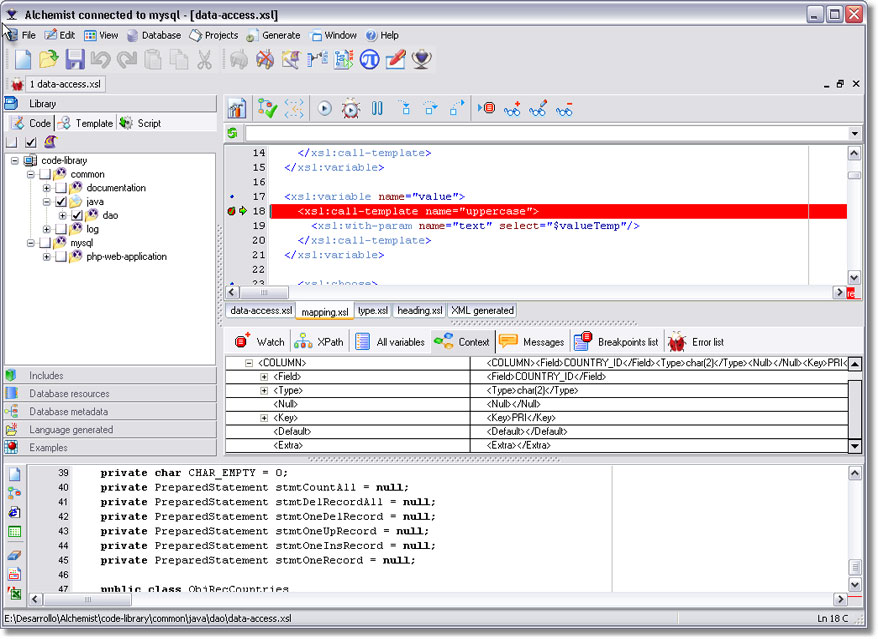
\includegraphics[scale=0.8]{pics/ide.eps}
\end{center}

\subsection{Software Development Tools}
\begin{center}
	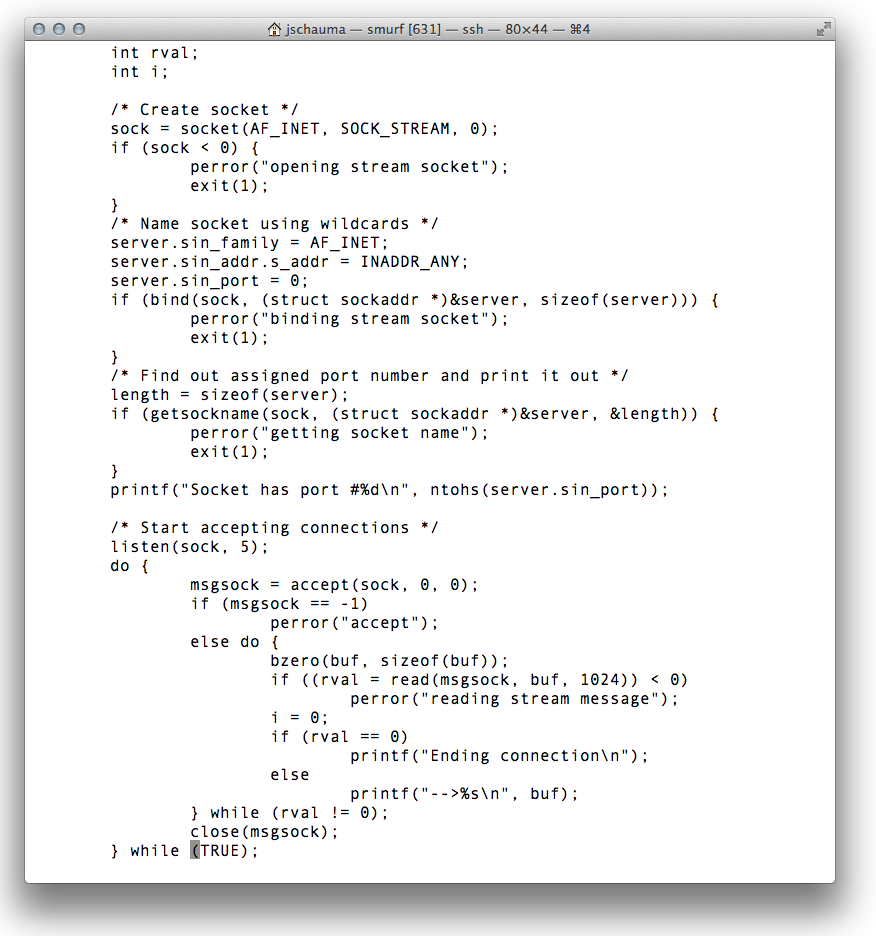
\includegraphics[scale=0.58]{pics/terminal.eps}
\end{center}

\subsection{Software Development Tools}
UNIX Userland is an IDE -- essential tools that follow the paradigm of ``Do
one thing, and do it right'' can be combined. \\

The most important tools are:
\begin{itemize}
	\item \verb+$EDITOR+
	\item the compiler toolchain
	\item {\tt gdb(1)} -- debugging your code
	\item {\tt make(1)} -- project build management, maintain program
		dependencies
	\item {\tt diff(1)} and {\tt patch(1)} -- report and apply differences
		between files
	\item {\tt cvs(1)}, {\tt svn(1)}, {\tt git(1)} etc. -- distributed project management,
		 version control
\end{itemize}

\subsection{Compilers}

\begin{center}
	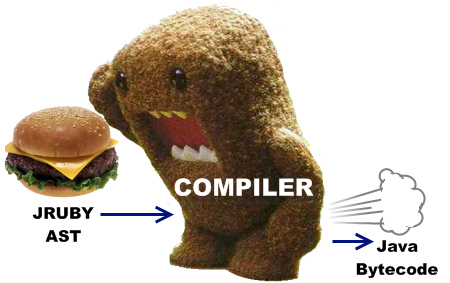
\includegraphics[scale=0.9,angle=-90]{pics/compiler_monster.eps}
\end{center}


\subsection{Compilers}

\begin{center}
	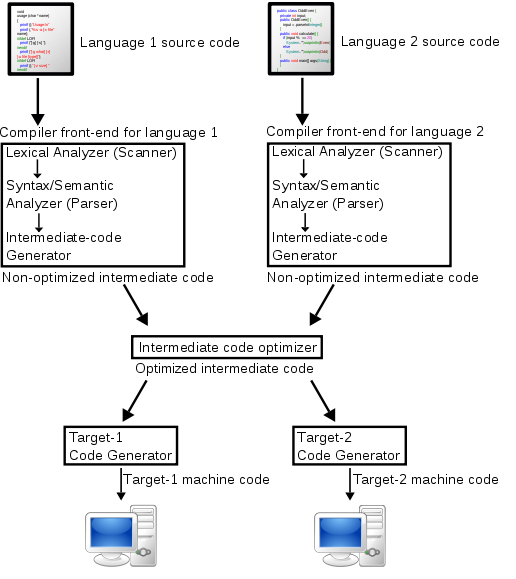
\includegraphics[scale=0.65]{pics/compiler.eps}
\end{center}

\subsection{Compilers}

A compiler translates {\em source code} from a high-level programming
language into {\em machine code} for a given architecture by performing a
number of steps:

\begin{itemize}
	\item lexical analysis
	\item preprocessing
	\item parsing
	\item semantic analysis
	\item code generation
	\item code optimization
\end{itemize}


\subsection{Compilers}

There are many different closed- and open-source compiler chains:

\begin{itemize}
	\item Intel C/C++ Compiler (or \verb+icc+)
	\item Turbo C / Turbo C++ / C++Builder (Borland)
	\item Microsoft Visual C++
	\item ...
\\

	\item Clang (a frontend to LLVM)
	\item GNU Compiler Collection (or \verb+gcc+)
	\item Portable C Compiler (or \verb+pcc+)
	\item ...
\end{itemize}

\subsection{The compiler toolchain}

The compiler usually performs preprocessing (via {\tt cpp(1)}), compilation
({\tt cc(1)}), assembly ({\tt as(1)}) and linking ({\tt ld(1)}).

\subsection{Preprocessing}

The compiler usually performs preprocessing (via {\tt cpp(1)}), compilation
({\tt cc(1)}), assembly ({\tt as(1)}) and linking ({\tt ld(1)}).

\begin{verbatim}
$ cd compilechain
$ cat hello.c
$ man cpp
$ cpp hello.c hello.i
$ file hello.i
$ man cc
$ cc -v -E hello.c > hello.i
$ more hello.i
$ cc -v -DFOOD=\"Avocado\" -E hello.c > hello.i.2
$ diff -bu hello.i hello.i.2
\end{verbatim}

\subsection{Compilation}

The compiler usually performs preprocessing (via {\tt cpp(1)}), compilation
({\tt cc(1)}), assembly ({\tt as(1)}) and linking ({\tt ld(1)}).

\begin{verbatim}
$ more hello.i
$ cc -v -S hello.i > hello.s
$ file hello.s
$ more hello.s
\end{verbatim}

\subsection{Assembly}

The compiler usually performs preprocessing (via {\tt cpp(1)}), compilation
({\tt cc(1)}), assembly ({\tt as(1)}) and linking ({\tt ld(1)}).

\begin{verbatim}
$ as -o hello.o hello.s
$ file hello.o
$ cc -v -c hello.s
$ objdump -d hello.o
[...]
\end{verbatim}

\subsection{Linking}

The compiler usually performs preprocessing (via {\tt cpp(1)}), compilation
({\tt cc(1)}), assembly ({\tt as(1)}) and linking ({\tt ld(1)}).

\begin{verbatim}
$ ld hello.o
[...]
$ ld hello.o -lc
[...]
$ cc -v hello.o
[...]
$ ld -dynamic-linker /lib64/ld-linux-x86-64.so.2 \
        /usr/lib/crt1.o /usr/lib/crti.o hello.o -lc /usr/lib/crtn.o
$ file a.out
$ ./a.out
\end{verbatim}

\subsection{Linking}

The compiler usually performs preprocessing (via {\tt cpp(1)}), compilation
({\tt cc(1)}), assembly ({\tt as(1)}) and linking ({\tt ld(1)}).

\begin{verbatim}
$ cc -v -DFOOD=\"Avocado\" hello.c 2>&1 | more
\end{verbatim}


\subsection{{\tt cc(1)} and {\tt ld(1)}}

The compiler usually performs preprocessing (via {\tt cpp(1)}), compilation
({\tt cc(1)}), assembly ({\tt as(1)}) and linking ({\tt ld(1)}).
\\

Different flags can be passed to {\tt cc(1)} to be passed through to each tool
as well as to affect all tools.  \\

\begin{verbatim}
$ cc -v -O2 -g hello.c 2>&1 | more
\end{verbatim}

\subsection{{\tt cc(1)} and {\tt ld(1)}}

The compiler usually performs preprocessing (via {\tt cpp(1)}), compilation
({\tt cc(1)}), assembly ({\tt as(1)}) and linking ({\tt ld(1)}).
\\

Different flags can be passed to {\tt cc(1)} to be passed through to each tool
as well as to affect all tools.  \\

The order of the command line flags {\em may} play a role!
Directories searched for libraries via {\tt -L} and the resolving of undefined
symbols via {\tt -l} are examples of position sensitive flags.
\\

\begin{verbatim}
$ cc -v main.c -L./lib2 -L./lib -lldtest 2>&1 | more


$ cc -v main.c -L./lib -L./lib2 -lldtest 2>&1 | more
\end{verbatim}


\subsection{{\tt cc(1)} and {\tt ld(1)}}

The compiler usually performs preprocessing (via {\tt cpp(1)}), compilation
({\tt cc(1)}), assembly ({\tt as(1)}) and linking ({\tt ld(1)}).
\\

Different flags can be passed to {\tt cc(1)} to be passed through to each tool
as well as to affect all tools.  \\

The order of the command line flags {\em may} play a role!
Directories searched for libraries via {\tt -L} and the resolving of undefined
symbols via {\tt -l} are examples of position sensitive flags.
\\

The behavior of the compiler toolchain may be influenced by environment
variables (eg {\tt TMPDIR}, {\tt SGI\_ABI}) and/or the compilers default
configuration file (MIPSPro's {\tt /etc/compiler.defaults} or gcc's {\tt
specs}).

\begin{verbatim}
$ cc -v hello.c
$ TMPDIR=/var/tmp cc -v hello.c
$ cc -dumpspec
\end{verbatim}

\subsection{{\tt make(1)}}

\begin{center}
	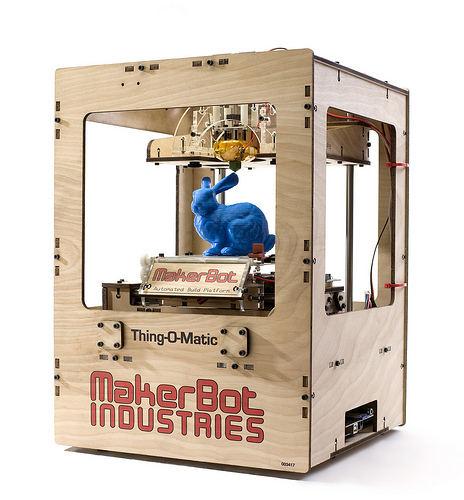
\includegraphics[scale=2.3]{pics/makerbot.eps}
\end{center}

\subsection{{\tt make(1)}}
{\tt make(1)} is a command generator and build utility. Using a
description file (usually {\em Makefile}) it creates a sequence of
commands for execution by the shell.

\begin{itemize}
	\item used to sort out dependency relations among files
\end{itemize}

\subsection{{\tt make(1)}}
{\tt make(1)} is a command generator and build utility. Using a
description file (usually {\em Makefile}) it creates a sequence of
commands for execution by the shell.

\begin{itemize}
	\item used to sort out dependency relations among files
	\item avoids having to rebuild the entire project after modification of a
		single source file
\end{itemize}

\subsection{{\tt make(1)}}
{\tt make(1)} is a command generator and build utility. Using a
description file (usually {\em Makefile}) it creates a sequence of
commands for execution by the shell.

\begin{itemize}
	\item used to sort out dependency relations among files
	\item avoids having to rebuild the entire project after modification of a
		single source file
	\item performs {\em selective} rebuilds following a {\em dependency graph}
\end{itemize}

\subsection{{\tt make(1)}}
{\tt make(1)} is a command generator and build utility. Using a
description file (usually {\em Makefile}) it creates a sequence of
commands for execution by the shell.

\begin{itemize}
	\item used to sort out dependency relations among files
	\item avoids having to rebuild the entire project after modification of a
		single source file
	\item performs {\em selective} rebuilds following a {\em dependency graph}
	\item allows simplification of rules through use of {\em macros} and {\em
		suffixes}, some of which are internally defined
\end{itemize}

\subsection{{\tt make(1)}}
{\tt make(1)} is a command generator and build utility. Using a
description file (usually {\em Makefile}) it creates a sequence of
commands for execution by the shell.

\begin{itemize}
	\item used to sort out dependency relations among files
	\item avoids having to rebuild the entire project after modification of a
		single source file
	\item performs {\em selective} rebuilds following a {\em dependency graph}
	\item allows simplification of rules through use of {\em macros} and {\em
		suffixes}, some of which are internally defined
	\item different versions of {\tt make(1)} (BSD make, GNU make, Sys V make,
		...) may differ (among other things) in
		\begin{itemize}
			\item variable assignment and expansion/substitution
			\item including other files
			\item flow control (for-loops, conditionals etc.)
		\end{itemize}
\end{itemize}

\subsection{{\tt make(1)}}

\begin{verbatim}
$ cd make-examples
$ ls *.[ch]
cmp.c       ls.c        main.c        stat_flags.c        util.c
extern.h    ls.h        print.c       stat_flags.h
\end{verbatim}

\begin{center}
	\includegraphics[scale=0.7,angle=-90]{pics/ls.eps}
\end{center}

\subsection{{\tt make(1)}}

\begin{verbatim}
$ cd make-examples
$ ls *.[ch]
cmp.c       ls.c        main.c        stat_flags.c        util.c
extern.h    ls.h        print.c       stat_flags.h
\end{verbatim}

\begin{center}
	\includegraphics[scale=0.7,angle=-90]{pics/ls-changed1.eps}
\end{center}

\subsection{{\tt make(1)}}

\begin{verbatim}
$ cd make-examples
$ ls *.[ch]
cmp.c       ls.c        main.c        stat_flags.c        util.c
extern.h    ls.h        print.c       stat_flags.h
\end{verbatim}

\begin{center}
	\includegraphics[scale=0.7,angle=-90]{pics/ls-changed2.eps}
\end{center}

\subsection{{\tt make(1)}}

\begin{verbatim}
$ cd make-examples
$ ls *.[ch]
cmp.c       ls.c        main.c        stat_flags.c        util.c
extern.h    ls.h        print.c       stat_flags.h
\end{verbatim}

\begin{center}
	\includegraphics[scale=0.7,angle=-90]{pics/ls-changed3.eps}
\end{center}

\subsection{{\tt make(1)}}

\begin{verbatim}
$ cd make-examples
$ ls *.[ch]
cmp.c       ls.c        main.c        stat_flags.c        util.c
extern.h    ls.h        print.c       stat_flags.h
\end{verbatim}

\begin{center}
	\includegraphics[scale=0.7,angle=-90]{pics/ls-changed4.eps}
\end{center}

\subsection{{\tt make(1)}}
\begin{verbatim}
$ make -f Makefile.1
cc -c cmp.c
cc -c ls.c
cc -c main.c
cc -c print.c
cc -c stat_flags.c
cc -c util.c
cc cmp.o ls.o main.o print.o stat_flags.o util.o -o ls
$ touch ls.h
$ make -f Makefile.1
cc -c cmp.c
cc -c ls.c
cc -c main.c
cc -c print.c
cc -c util.c
cc cmp.o ls.o main.o print.o stat_flags.o util.o -o ls
$
\end{verbatim}

\subsection{{\tt make(1)}}
\begin{verbatim}
$ make -f Makefile.2
cc    -c -o cmp.o cmp.c
cc    -c -o ls.o ls.c
[...]
cc    -c -o util.o util.c
ls depends on cmp.o ls.o main.o print.o stat_flags.o util.o
cc  cmp.o ls.o main.o print.o stat_flags.o util.o -o ls
$ bmake -f Makefile.2
gcc -pipe -O2  -c cmp.c
gcc -pipe -O2  -c ls.c
[...]
gcc -pipe -O2  -c util.c
ls depends on cmp.o ls.o main.o print.o stat_flags.o util.o
gcc  cmp.o ls.o main.o print.o stat_flags.o util.o -o ls
$
\end{verbatim}

\subsection{{\tt make(1)}}
\begin{verbatim}
$ make -f Makefile.3
cc -c cmp.c -o cmp.b
cc -c ls.c -o ls.b
cc -c main.c -o main.b
cc -c print.c -o print.b
cc -Wall -g -c stat_flags.c -o stat_flags.bar
cc -Wall -g -c util.c -o util.bar
ls depends on cmp.b ls.b main.b print.b stat_flags.bar util.bar
cc  cmp.b ls.b main.b print.b stat_flags.bar util.bar -o ls
$
\end{verbatim}


\subsection{Priority of Macro Assignments for {\tt make(1)}}

\begin{enumerate}
	\item Internal (default) definitions of {\tt make(1)}
	\item Current shell environment variables.  This includes macros that you
		enter on the {\em make} command line itself.
	\item Macro definitions in {\em Makefile}.
	\item Macros entered on the {\tt make(1)} command line, if they follow
		the {\em make} command itself.
\end{enumerate}

\subsection{{\tt make(1)}}

\begin{verbatim}
$ bmake -f Makefile.4
[...]
$ bmake -f Makefile.2
[...]
$ CFLAGS=-Werror bmake -f Makefile.2
[...]
$ CFLAGS=-Werror bmake -f Makefile.4
[...]
$ bmake CFLAGS=-Werror -f Makefile.2
[...]
$ bmake CFLAGS=-Werror -f Makefile.4
[...]
\end{verbatim}

\subsection{Ed is the standard text editor.}
\begin{verbatim}
$ ed
?
help
?
quit
?
exit
?
bye
?
eat flaming death
?
^C
?
^D
?
\end{verbatim}

\subsection{Ed is the standard text editor.}
\begin{verbatim}
$ ed
a
ed is the standard Unix text editor.
This is line number two.
.
2i

.
%l
3s/two/three/
w foo
q
$ cat foo
\end{verbatim}

\subsection{{\tt diff(1)} and {\tt patch(1)}}
{\tt diff(1)}:
\begin{itemize}
	\item compares files line by line
	\item output may be used to automatically edit a file
	\item can produce human ``readable'' output as well as diff entire
		directory structures
	\item output called a {\em patch}
\end{itemize}

\subsection{{\tt diff(1)} and {\tt patch(1)}}
{\tt patch(1)}:
\begin{itemize}
	\item applies a {\tt diff(1)} file (aka {\em patch}) to an original
	\item may back up original file
	\item may guess correct format
	\item ignores leading or trailing ``garbage''
	\item allows for reversing the patch
	\item may even correct context line numbers
\end{itemize}

\subsection{{\tt diff(1)} and {\tt patch(1)}}
\begin{verbatim}
$ diff Makefile.2 Makefile.4
8c8
< #CFLAGS=	-Wall -g
---
> CFLAGS=	-Wall -g
$ cp Makefile.2 /tmp
$ ( diff -e Makefile.2 Makefile.4; echo w; ) | ed Makefile.2
$ diff Makefile.[24]
$ mv /tmp/Makefile.2 .
$ diff -c Makefile.[24]
$ diff -u Makefile.[24] > /tmp/patch
$ patch </tmp/patch
$ diff Makefile.[24]
\end{verbatim}

\subsection{A Debugger}
\vspace*{\fill}
\begin{center}
	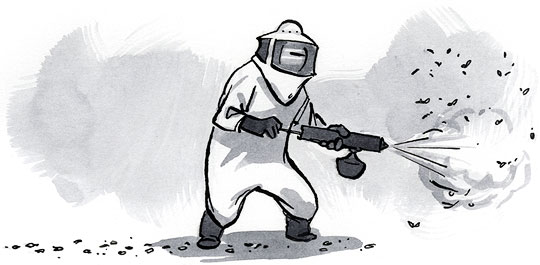
\includegraphics{pics/debugging.eps}
\end{center}
\vspace*{\fill}

\subsection{{\tt gdb(1)}}

The purpose of a debugger such as {\tt gdb(1)} is to allow you to see what is
going on ``inside'' another program while it executes -- or what another
program was doing at the moment it crashed. {\tt gdb} allows you to

\begin{itemize}
	\item make your program stop on specified conditions (for example by
		setting {\em breakpoints})
	\item examine what has happened, when your program has stopped (by looking
		at the {\em backtrace}, inspecting the value of certain variables)
	\item inspect control flow (for example by {\em stepping} through the
		program)
\end{itemize}
\vspace{.25in}
Other interesting things you can do:

\begin{itemize}
	\item examine stack frames: {\em info frame}, {\em info locals}, {\em info
		args}
	\item examine memory: {\em x}
	\item examine assembly: {\em disassemble func}
\end{itemize}

\subsection{{\tt gdb(1)}}
\begin{verbatim}
$ cc -g gdb1.c
$ ./a.out
[...]
$ gdb ./a.out
[...]
frame 8
print c
n
n
[...]
li

\end{verbatim}

\subsection{{\tt gdb(1)}}
\begin{verbatim}
$ ulimit -c unlimited
$ cc -g gdb2.c
$ ./a.out
$ gdb a.out core
bt
[...]
frame 2
li
p buf
kill
break gdb2.c:main
run
li
n
p buf
p num
\end{verbatim}

\subsection{Revision Control}
Version control systems allow you to

\begin{itemize}
	\item collaborate with others
	\item simultaneously work on a code base
	\item keep old versions of files
	\item keep a log of the who, when, what, and why of any changes
	\item perform release engineering by creating {\em branches}
\end{itemize}

\subsection{Revision Control}
\begin{itemize}
	\item Source Code Control System ({\em SSCS}) begat the Revision
		Control System ({\em RCS}).
	\item RCS operates on a single file; still in use for misc. OS
		config files
	\item the Concurrent Versions System ({\em CVS}) introduces a
		client-server architecture, control of hierarchies
	\item {\em Subversion} provides atomic commits, renaming, cheap
		branching etc.
	\item {\em Git}, {\em Mercurial} etc. implement a {\em
		distributed} approach (ie peer-to-peer versus
		client-server), adding other features (cryptographic
		authentication of history, ...)
\end{itemize}

\subsection{Revision Control}
Examples:

{\tt http://cvsweb.netbsd.org/bsdweb.cgi/src/bin/ls/} \\

{\tt http://svnweb.freebsd.org/base/stable/9/bin/ls/} \\

{\tt http://git.savannah.gnu.org/cgit/coreutils.git/log/}

\subsection{Setting up git(1) for your final project}
Initialize the source code repository:
\\

\begin{verbatim}
ssh linux-lab.cs.stevens.edu
mkdir -p ~/git/sws.git
cd ~/git/sws
git --bare init
\end{verbatim}

\subsection{Setting up git(1) for your final project}
Add your code from the project directory:
\\

\begin{verbatim}
ssh linux-lab.cs.stevens.edu
cd ~/cs631/sws
git init
git remote add origin ~/git/sws.git
git config branch.master.merge refs/heads/master
git config branch.master.remote origin
git config --global user.name "Your Full Name"
git config --global user.email $USER@stevens.edu
git add *
git commit -m "initial import of all files"
git push origin master
\end{verbatim}

\subsection{Setting up git(1) for your final project}
Check out a copy on a local host and make changes:
\\

\begin{verbatim}
local$ git clone linux-lab.cs.stevens.edu:git/sws.git
local$ cd sws
local$ $EDITOR README
local$ git add README
local$ git commit README
local$ git push

linux-lab$ cd ~/cs631/sws
linux-lab$ git pull
linux-lab$ $EDITOR ...
linux-lab$ git add ...; git commit; git push
\end{verbatim}

\subsection{Homework}
Generate an ssh key pair and send me the {\em public} key. \\
See {\tt ssh-keygen(1)}.

\subsection{Links}
Revision Control: \\
{\tt http://cvsbook.red-bean.com/cvsbook.html} \\

{\tt http://svnbook.red-bean.com/} \\

{\tt http://git-scm.com/} \\

GDB: \\
{\tt http://sources.redhat.com/gdb/current/onlinedocs/gdb\_toc.html} \\

\verb+http://heather.cs.ucdavis.edu/~matloff/UnixAndC/CLanguage/Debug.html+ \\

{\tt http://www.unknownroad.com/rtfm/gdbtut/gdbtoc.html}


\end{document}
